\section{Numerical stability}
The following section will give a brief insight in to the effects of choosing different $\theta$ values in the $\theta-$scheme. The benchmark tests FSI-2 and FSI-3, discussed in the previous section has been used since they known to blow up with certain values of $\theta$ and $\Delta t$. Only the effects of Drag as been studied as the three other quantities shows the same behavior.   The impact of choosing different $\theta$ values for energy stability in the solid mechanical case CSM1 is also discussed.

\begin{figure}[H]  \label{fig:FSI2drag_plots} 
  \caption {Drag for FSI2 with $\Delta t = 0.01$ with different values for $\theta$}
  \begin{minipage}[b]{0.6\linewidth}
    \centering
    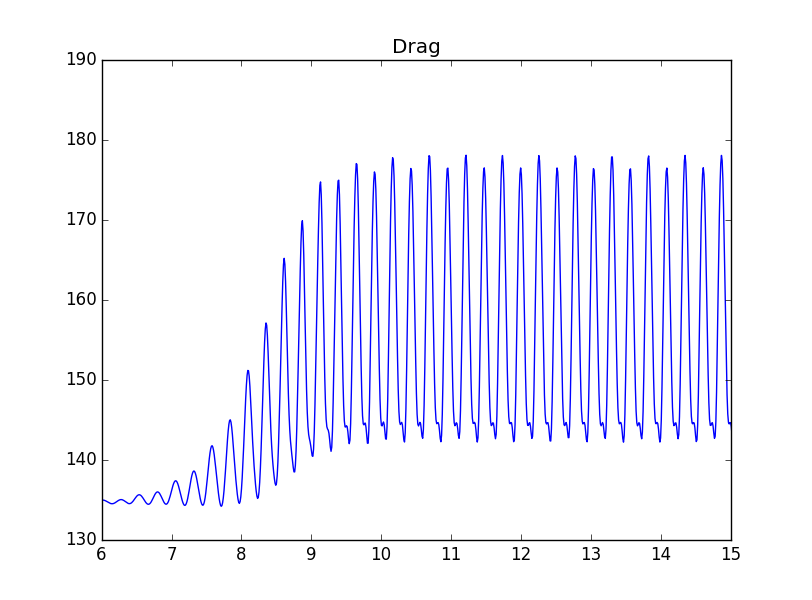
\includegraphics[scale=0.40]{./Temporal_stability/FSI2_001_051_big.png} 
    \caption{$\theta = 0.51 $} 
    \vspace{4ex}
  \end{minipage}%%
  \begin{minipage}[b]{0.6\linewidth}
    \centering
    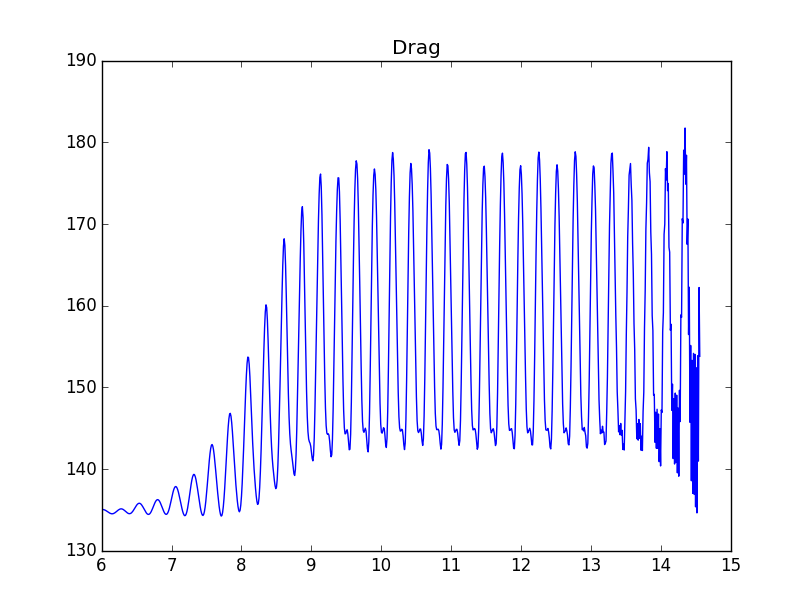
\includegraphics[scale=0.40]{./Temporal_stability/FSI2_001_050_big.png} 
    \caption{$\theta = 0.50 $} 
    \vspace{4ex}
  \end{minipage} 
  \begin{minipage}[b]{0.6\linewidth}
    \centering
    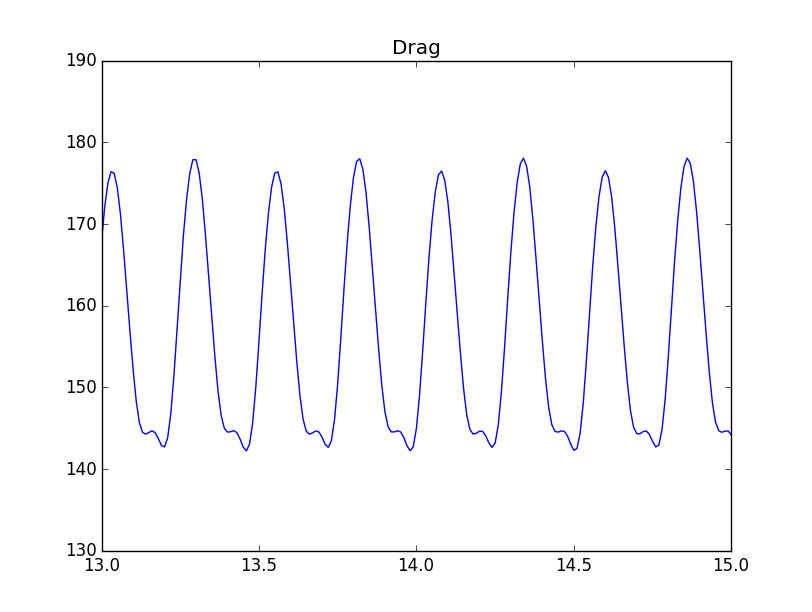
\includegraphics[scale=0.40]{./Temporal_stability/FSI2_001_051_small.png} 
    \caption{$\theta = 0.51 $} 
    \vspace{4ex}
  \end{minipage}%% 
  \begin{minipage}[b]{0.6\linewidth}
    \centering
    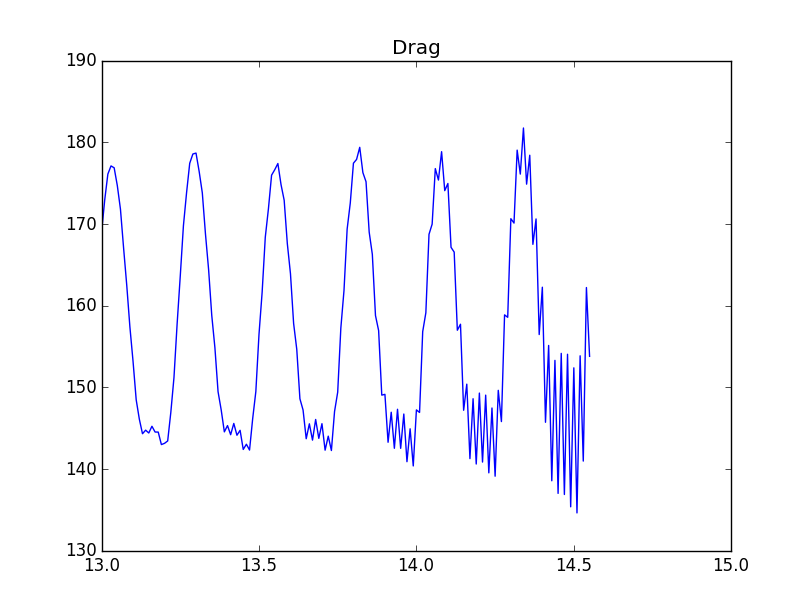
\includegraphics[scale=0.40]{./Temporal_stability/FSI2_001_050_small.png} 
    \caption{$\theta = 0.50 $} 
    \vspace{4ex}
  \end{minipage} 
\end{figure}

\ref{fig:FSI2drag_plots} show the plots of Drag with $\Delta t = 0.01$, showing the instability when choosing $\theta = 0.5$. The Crank-Nicholson scheme is stable until about 13 seconds where we see that it blows up and the solver diverges. While the shifted Crank-Nicholson, $\theta = 0.5 + \Delta t$, is stable throughout the computing time.\newline

\begin{figure}[H]  \label{fig:CSM3_dis_plots} 
   \caption {CSM3 displacements with $\Delta t = 0.01$ with different values for $\theta$}
  \begin{minipage}[b]{0.6\linewidth}
    \centering
    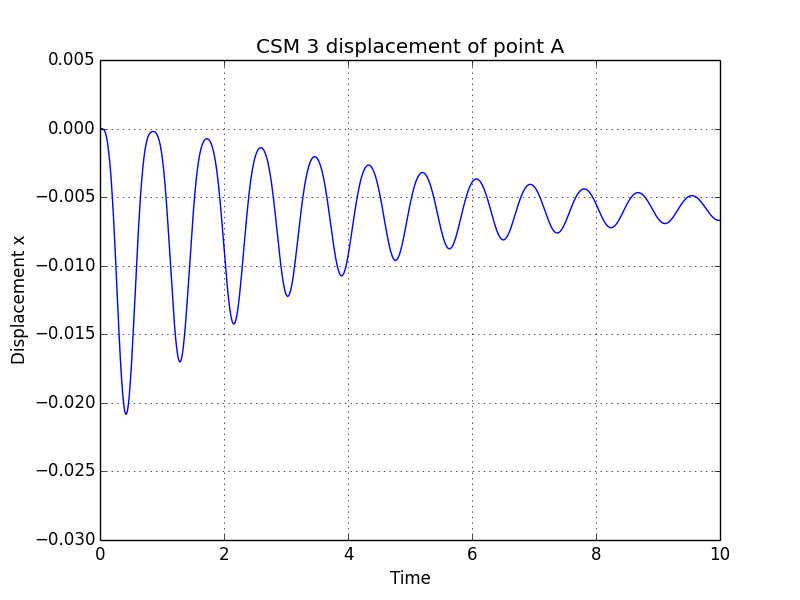
\includegraphics[scale=0.40]{./Temporal_stability/CSM3_implicit.png} 
    \caption{$\theta = 1 $} 
    \vspace{4ex}
  \end{minipage}%%
  \begin{minipage}[b]{0.6\linewidth}
    \centering
    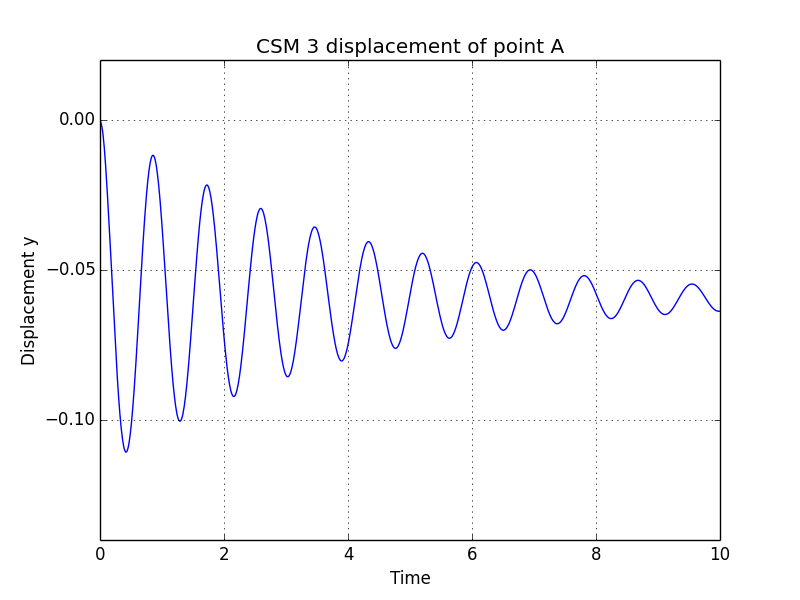
\includegraphics[scale=0.40]{./Temporal_stability/CSM3_implicit_y.png} 
    \caption{$\theta = 1 $} 
    \vspace{4ex}
  \end{minipage} 
  \begin{minipage}[b]{0.6\linewidth}
    \centering
    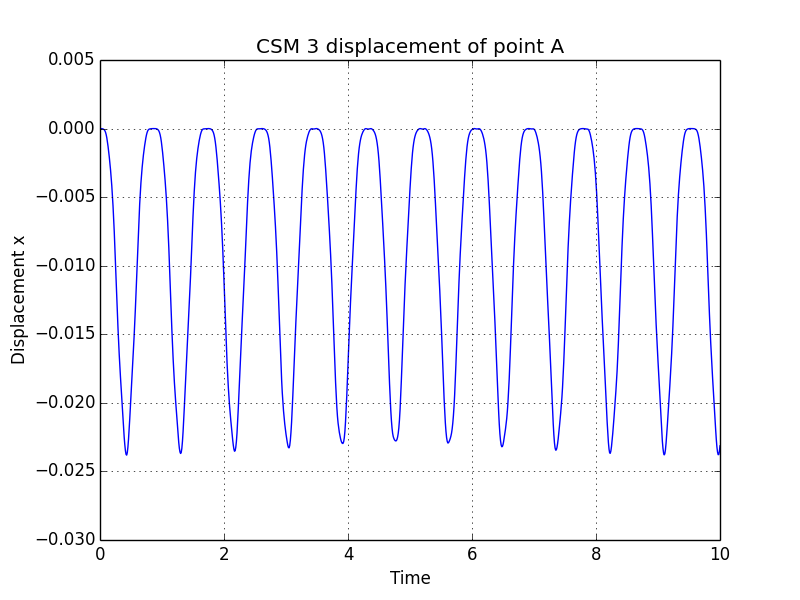
\includegraphics[scale=0.40]{./Temporal_stability/CSM3_Crank.png} 
    \caption{$\theta = 0.5 $} 
    \vspace{4ex}
  \end{minipage}%% 
  \begin{minipage}[b]{0.6\linewidth}
    \centering
    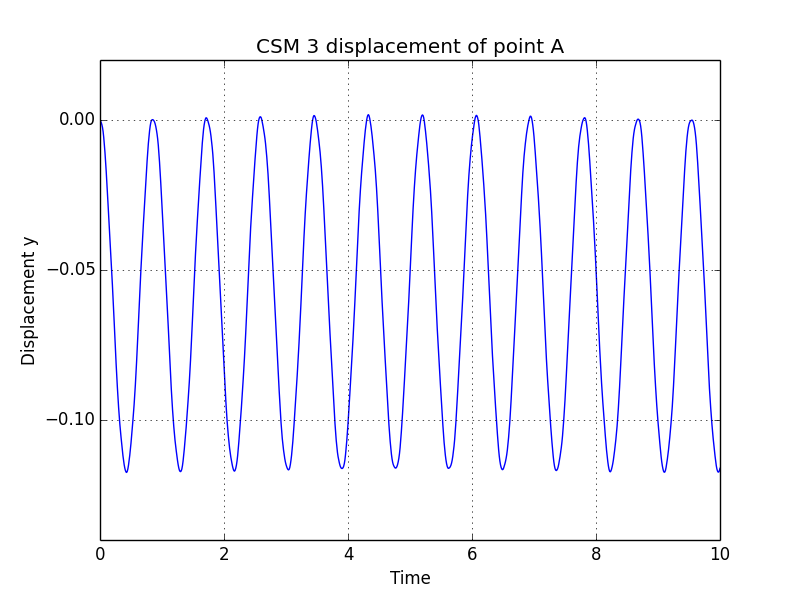
\includegraphics[scale=0.40]{./Temporal_stability/CSM3_Crank_y.png} 
    \caption{$\theta = 0.5 $} 
    \vspace{4ex}
  \end{minipage} 
\end{figure}
Figure \ref{fig:CSM3_dis_plots} shows plots of the displacements in x and y directions for $\theta = 0.5$ and $1$. With the implicit scheme ($\theta=1$) the bar moves to a steady state solution. This means energy has not been preserved and the energy dissipates. While in the Crank-Nicholson scheme ($\theta = 0.5$)

\subsubsection*{Comments on numerical stability}
The shifted version of the Crank-Nicholson scheme is stable when computing for time step values as low as $\Delta t = 0.01$. However for $\Delta t = 0.001$ the normal Crank-Nicholson scheme ($\theta =0.5$) can be used and i long term stabile. It has also been reported in \cite{Wick2011} that the Crank-Nicholson, $\theta = 0.5$, scheme is stable throughout the computing time by setting $\Delta t = 0.001$.



